\chapter{Conclusion et perspectives}
\paragraph{}
Comme toute étude de recherche, les portes sont toujours ouvertes pour des améliorations et des adaptations. Notre logiciel est disponible sur le gestionnaire de version GitHub en version open source sur mon compte\footnote{https://github.com/metanote/Extraction} ce qui permet d'ouvrir les pistes à d'autres personnes pour l'utiliser et l'améliorer. 
\section*{Améliorations possibles}
\paragraph{}
Ce logiciel est un outil d'extraction de propriétés à partir de DBpédia, permet d'annotés temporellement des triplets DBpedia. Actuellement, cet outil dépend de l'avis d'un expert pour valider les résultats de notre algorithme. Il serait intéressant de rendre toute cette procédure de modélisation automatique. Aussi, on peut intégrer une procédure d'apprentissage, en cherchant à classifier les propriétés DBpédia sous forme de deux classes par exemple (PropWithResult, PropWithoutResult) avec un algorithme d'apprentissage automatique comme (SVM ou Adaboost) pour la procédure de validation.
\subparagraph{}
Dans cette étude, nous avons travaillé avec deux indices temporels (Date, Year). Nous pouvons chercher d'autres indices qui peuvent nous aider à repérer plus de propriétés temporelles dans DBpédia. Nous avons tourné notre algorithme sur $1992$ propriétés DBpédia que nous avons extrait. Il serait intéressant de tourner cet algorithme sur une autre base de faits qui contient de propriétés DBpedia.
Nous avons développé un prototype dans lequel nous avons cherché seulement les propriétés qui dépendent d'un point de temps particulier.
Dans notre hypothèse de base, nous voulons aussi chercher les propriétés qui sont vraies dans un intervalle de temps, des propriétés temporelles comme (MotifStartDate,MotifEndDate), mais dans le fichier de propriétés DBpedia nous avons repéré seulement $7$ couples de propriétés qui vérifie cette condition. Cela donne seulement $7$ intervalles de temps possibles sur $1992$.
\subparagraph{}
La procédure de la fouille est intéressante pour une quantité de données de masse. Nous avons formé avec les motifs temporels (Year, Date) $305$ couples de propriétés à partir de $1992$ propriétés. Sur les $20$ première couple de propriétés nous avons trouvé $4$ qui donnent des quadruplets valides. Avec une parcours aléatoire de la liste de couples, nous avons récupéré $35$ fichiers de triplets annotés dans le fichier $historic.csv$.
\paragraph{}
Aussi, nous pouvons chercher que les triplets qu'on veut annoter dans DBpédia sous forme d'une liste, puis à partir des faits trouver dans ces triplets. Ensuite, nous cherchons leurs annotations temporels dans les dumps de Wikipédia et Wikidata.
\paragraph{}
Il est intéressent de fusionner deux triplets afin d'avoir un seul plus structuré. La représentation de connaissances sous forme de triplets, nous permet non seulement de les reutiliser dans des divers type de traitement, mais aussi de faire des déductions à partir de ces triplets pour exprimer d'autres concepts. Nous avons remarqué aussi que la modélisation des connaissances permet de rendre les informations plus utiles et elle peut éviter beaucoup de redondances. 
\subparagraph{}
Actuellement on parle plus de l'énorme quantité de données ou les données massives $Big$ $Data$ sur le Web. Derrière ces mots se cachent l’incroyable quantité de données disponible notamment sur le net, et surtout la manière dont on peut les traiter pour obtenir des informations utiles. On se rend compte de la mauvaise gestion, la duplication, la perte de l'information et la difficulté liée à la recherche de ces informations. C'est pour cela, nous cherchons toujours à optimiser l'usage de ces métadonnées et structuré les données sur le Web.
\subparagraph{}
D'après une étude faite par EMC\footnote{http://www.emc.com/leadership/digital-universe/index.htm}{\it the digital universe study with  reasearch and analysis by IDC}, la firme IDC\footnote{http://www.idc.fr/}, mandatée par EMC (spécialiste des logiciels et systèmes de stockage), a réalisé une étude sur la prolifération de ces données et anticipe déjà ce que cela donnera en $2020$. Les résultats sont particulièrement intéressants. Voici les principaux enseignements :
\begin{itemize}
\item En $2011$, $5$ exaoctets de données étaient générés tous les deux jours. Cela se fait désormais en $10$ minutes seulement.
\item Seules $0,5$\% de ces données sont analysées
\item Il n’y avait que $130$ exaoctets de données dans l’univers numérique en $2005$. Il devrait y en avoir plus de $40 000$ à l’horizon $2020$.
\item En $2020$, les données représenteront l’équivalent de plus de $5 000$ GO par personne.
\item En $2012$, $35$\% de ces informations nécessiterait une protection, mais ce n’est le cas que pour $20$\% d’entre elles.
\end{itemize}
\begin{figure}[H]
        \centering
                \centering
                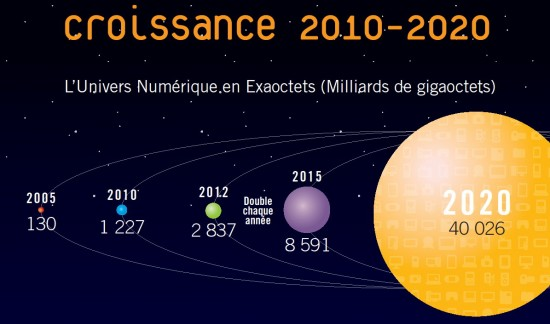
\includegraphics[width=10cm]{datas.jpg}
               \caption{L'univers des données}

\end{figure}
\paragraph{}
Le besoin de gérer des données extrêmement volumineuses est flagrant. Les outils utilisés ne sont pas en adéquation avec les volumes de données engendrés dans l'exploration de Big Data, la National Security Agency (NSA) est actuellement en train de construire le Utah Data Center. Ce Data Center pourra collecter une masse gigantesque d'information pour des analyses, recherches et surveillance. Les données seront le pétrole de l'avenir. La modélisation et la gestion de ces données seront le plus grand défie de l'informatique intelligent dans les prochaines années. 
\newpage
\section*{Conclusion}
\paragraph{}
Le stage réalisé a été enrichissant de plusieurs façons. En effet, bien que ce stage soit un stage orienté recherche, il comporte de nombreux aspects d'ingénierie. Les recherches effectuées sont des réponses aux besoins qui ont été accordées dans d'autres travaux de recherche sur l'annotation temporelle des triplets RDF et qui est aussi qui est lié aux travaux de mes tuteurs de stage. Les réponses sont également dirigées vers du concret notamment l'élaboration d'une application Java. Cette dualité recherche-ingénierie a été motivante et m'a permis d'affiner une certaine ouverture d'esprit et d'améliorer mes connaissances dans le domaine du Web sémantique.
\subparagraph{}
En plus, durant ce stage, j'ai assisté des présentations dans les domaines du Web sémantique et Big Data. Cela m'a permis de voir les études et les travaux dans ces domaines. La rencontre de différentes visions est toujours intéressante et a permis dans ce cas de situer l'informatique et l'utilisation. Par ailleurs, le travail dans un milieu de recherche m'a permis de chercher des réponses à des questions et résoudre des problématiques intéressantes.
\subparagraph{}
Enfin, l'étude d'annotation temporelle des données DBpédia m'a permis d'approfondir mes connaissances dans le domaine du Web sémantique et de prendre conscience de son importance. Je suis dorénavant intimement convaincu que les recherches dans le Web sémantique vont permettre d'évoluer le Web et de concrétiser la vision de Tim Berners-Lee.   
